\documentclass[11pt, onesided]{book}

%%%%%%%%%%%%%%Include Packages%%%%%%%%%%%%%%%%%%%%%%%%%%
\usepackage{xcolor}
\usepackage{mathtools}
\usepackage[a4paper, total={6in, 8in}, margin=1.25in]{geometry}
\usepackage{amsmath}
\usepackage{amssymb}
\usepackage{paralist}
\usepackage{rsfso}
\usepackage{amsthm}
\usepackage{wasysym}
\usepackage[inline]{enumitem}   
\usepackage{hyperref}
\usepackage{tocloft}
\usepackage{titlesec}
\usepackage{colortbl}
%%%%%%%%%%%%%%%%%%%%%%%%%%%%%%%%%%%%%%%%%%%%%%%%%%%%%%%%


%%%%%%%%%%%%%%%Chapter Setting%%%%%%%%%%%%%%%%%%%%%%%%%%
\definecolor{gray75}{gray}{0.75}
\newcommand{\hsp}{\hspace{20pt}}
\titleformat{\chapter}[hang]{\Huge\bfseries}{\thechapter\hsp\textcolor{gray75}{$\mid$}\hsp}{0pt}{\Huge\bfseries}
%%%%%%%%%%%%%%%%%%%%%%%%%%%%%%%%%%%%%%%%%%%%%%%%%%%%%%%%

%%%%%%%%%%%%%%%%%Theorem environments%%%%%%%%%%%%%%%%%%%
\newtheoremstyle{break}
  {\topsep}{\topsep}%
  {\itshape}{}%
  {\bfseries}{}%
  {\newline}{}%
\theoremstyle{break}
\theoremstyle{break}
\newtheorem{axiom}{Axiom}
\newtheorem{thm}{Theorem}[section]
\renewcommand{\thethm}{\arabic{section}.\arabic{thm}}
\newtheorem{lem}{Lemma}[thm]
\newtheorem{cor}{Corollary}[thm]
\newtheorem{defn}{Definition}[thm]
\newenvironment{indEnv}[1][Proof]
  {\proof[#1]\leftskip=1cm\rightskip=1cm}
  {\endproof}
%%%%%%%%%%%%%%%%%%%%%%%%%%%%%%%%%%%%%%%%%%%%%%%%%%%%%%


%%%%%%%%%%%%%%%%%%%%%%%Integral%%%%%%%%%%%%%%%%%%%%%%%
\def\upint{\mathchoice%
    {\mkern13mu\overline{\vphantom{\intop}\mkern7mu}\mkern-20mu}%
    {\mkern7mu\overline{\vphantom{\intop}\mkern7mu}\mkern-14mu}%
    {\mkern7mu\overline{\vphantom{\intop}\mkern7mu}\mkern-14mu}%
    {\mkern7mu\overline{\vphantom{\intop}\mkern7mu}\mkern-14mu}%
  \int}
\def\lowint{\mkern3mu\underline{\vphantom{\intop}\mkern7mu}\mkern-10mu\int}
%%%%%%%%%%%%%%%%%%%%%%%%%%%%%%%%%%%%%%%%%%%%%%%%%%%%%%



\newcommand{\R}{\mathbb{R}}
\newcommand{\N}{\mathbb{N}}
\newcommand{\Z}{\mathbb{Z}}
\newcommand{\Q}{\mathbb{Q}}
\newcommand{\C}{\mathbb{C}}
\newcommand{\Power}{\mathcal{P}}
\newcommand{\ee}[1]{\cdot 10^{#1}}
\newcommand{\spa}{\text{span}}
\newcommand{\sgn}{\text{sgn}}
\newcommand{\degr}{\text{deg}}
\newcommand{\pd}{\partial}
\newcommand{\that}[1]{\widetilde{#1}}
\newcommand{\lr}[1]{\left(#1\right)}
\newcommand{\vmat}[1]{\begin{vmatrix} #1 \end{vmatrix}}
\newcommand{\bmat}[1]{\begin{bmatrix} #1 \end{bmatrix}}
\newcommand{\pmat}[1]{\begin{pmatrix} #1 \end{pmatrix}}
\newcommand{\rref}{\xrightarrow{\text{row\ reduce}}}
\newcommand{\txtarrow}[1]{\xrightarrow{\text{#1}}}
\newcommand{\txt}{Wald's \textit{General Relativity}}

\newcommand{\note}{\color{red}Note: \color{black}}
\newcommand{\remark}{\color{blue}Remark: \color{black}}
\newcommand{\example}{\color{green}Example: \color{black}}
\newcommand{\exercise}{\color{green}Exercise: \color{black}}

%%%%%%%%%%%%%table of contents%%%%%%%%%%%%%%%%%%%%%%%%%%%%
%\setlength{\cftchapindent}{0em}
%\cftsetindents{section}{2em}{3em}
%
%\renewcommand\cfttoctitlefont{\hfill\huge\bfseries}
%\renewcommand\cftaftertoctitle{\hfill\mbox{}}
%
%\setcounter{tocdepth}{2}
%%%%%%%%%%%%%%%%%%%%%%%%%%%%%%%%%%%%%%%%%%%%%%%%%%%%%%%%%%


%%%%%%%%%%%%%%%%%%%%%Footnotes%%%%%%%%%%%%%%%%%%%%%%%%%%%
\newcommand\blfootnote[1]{%
  \begingroup
  \renewcommand\thefootnote{}\footnote{#1}%
  \addtocounter{footnote}{-1}%
  \endgroup
}
%%%%%%%%%%%%%%%%%%%%%%%%%%%%%%%%%%%%%%%%%%%%%%%%%%%%%%%%%

%%%%%%%%%%%%%%%%%%%%%Section%%%%%%%%%%%%%%%%%%%%%%%%%%%%%
\makeatletter
\def\@seccntformat#1{%
  \expandafter\ifx\csname c@#1\endcsname\c@section\else
  \csname the#1\endcsname\quad
  \fi}
\makeatother
%%%%%%%%%%%%%%%%%%%%%%%%%%%%%%%%%%%%%%%%%%%%%%%%%%%%%%%%%

\begin{document}
\tableofcontents

\newpage
\chapter{-}
\section{First and Second Quantization Schemes}
We are familiar with the first quantization scheme, for instance, for describing an electron in a Hydrogen atom, the Hamiltonian is 
\begin{align*}
H =  -\frac{\hbar^2}{2m}\nabla^2 - \frac{e^2}{4\pi \epsilon_0 r}\,.
\end{align*}
The energy eigenstates $|\psi_n\rangle$ of such a Hamiltonian form a basis for the quantum states of the electron. We can then apply other operators, such as $\hat{x}$ and $\hat{p}$ to find the expectation values $\langle \psi | \hat{x}|\psi\rangle$ and $\langle \psi |\hat{p}|\psi\rangle$. The steps that we take in the computation of those expectation values depend on what picture (Schrodinger picture or Heisenberg picture) we are using. This summarizes the first quantization scheme.\\

Notice that, first quantization scheme describes a fixed number of particles (such as only one electron in the Hydrogen model). The quantum state (of the electron in the Hydrogen model) can usually be expressed using a wavefunction $\langle x | \psi\rangle$ living in the real space. Operators act on coordinates of the wavefunction, that is, for instance
\begin{align*}
\langle \hat{p}\rangle = \langle \psi | \hat{p}|\psi\rangle = \int dx \, \langle \psi | x\rangle \langle x | \hat{p} |\psi\rangle\,.
\end{align*}
It is natural to use the first quantization scheme to describe single-particle physics, but when it comes to many-body physics, or particle number becomes a variable, we might encounter issues such as dealing with the exchange of particles. In many-body first-quantization quantum mechanics, the wavefunction of the system is usually expressed as a Slater determinant, 
\begin{align*}
\psi(\vec{r}_1, \vec{r}_2,\cdots ) = \frac{1}{\sqrt{N!}} \vmat{\phi_1(\vec{r}_1) & \phi_1(\vec{r}_2) & \cdots & \phi_1(\vec{r}_N) \\
\phi_2(\vec{r}_1) & \phi_2(\vec{r}_2) & \cdots & \phi_2(\vec{r}_N) \\
\vdots & \vdots & \ddots & \vdots\\
\phi_N(\vec{r}_1) & \phi_N(\vec{r}_2) & \cdots & \phi_N(\vec{r}_N) }_\pm
\end{align*}
with $\phi_i(\vec{r}_j)$ being single-particle wavefunction of the $i$-th particle. The use of this wavefunction is often cumbersome.\\

In the language of second quantization scheme, instead of fixing the particle number, we allow it to be a variable. 	In this case, the quantum states keep track of the occupation of, for instance, single-particle Hamiltonian energy levels, that is, 
\begin{align*}
\{|n_1, n_2, \cdots\rangle| \, n_i \text{ denotes the $i$-th level occupation, }\sum_i n_i = \text{total particle number}\}
\end{align*}
spans the Fock space $\mathbb{F}$, which is the space for one specie of identical particle, 
\begin{align*}
\mathbb{F} = \bigoplus_{N=0}^\infty \mathbb{F}_N
\end{align*}
with $\mathbb{F}_N$ being Hilbert space for $N$-identical particles. We note here that the energy levels (with $n_i$ denoting their occupation particle numbers) do not have to be single-particle Hamiltonian energy levels, they can also be the energy levels of the multiparticle system that we are interested in (see the SSH model that we will discuss in the following). The first kind of operators that we shall define in the language of second quantization scheme is the creation and annihilation operators, $\hat{a}$ and $\hat{a}^\dagger$, such that 
\begin{align*}
&\hat{a}^\dagger_i|\cdots, n_i, \cdots\rangle = \sqrt{n_i+1}|\cdots, n_i+1,\cdots\rangle\,,\\
&\hat{a}_i | \cdots, n_i, \cdots\rangle = \begin{cases}
\sqrt{n_i}| \cdots, n_i-1,\cdots\rangle & n_i \neq 0\\
0 & n_i =0 \end{cases} \,,
\end{align*}
with a commutation relation $[\hat{a}_i, \hat{a}_j^\dagger] = \delta_{ij}$ (commutation relation for bosons, and anticommutation relation for fermions). \\

Then we shall introduce the field operators. In position space representation with any single-particle basis $\{\phi_i (\vec{r})\}$,
\begin{align*}
\hat{\psi}(\vec{r}) =\sum_i \phi_i(\vec{r}) \, \hat{a}_i \,,\qquad
\hat{\psi}^\dagger(\vec{r}) = \sum_i \phi_i^*(\vec{r}) \, \hat{a}^\dagger_i\,,
\end{align*}
where in particular, $\phi_i(\vec{r}_j)$ is a single-particle wavefunction. The field operators can be understood as physically creating or removing a particle at some position. It also follows immediately that the field operators satisfy $[\hat{\psi}(\vec{r}),\, \hat{\psi}(\vec{r}') ] = \delta(\vec{r}-\vec{r}')$ (commutation relation for bosons, and anticommutation relation for fermions). It can be seen from here that, if we choose the plane-wave basis
\begin{align*}
\phi_{\vec{k}}(\vec{r}) = \frac{1}{\sqrt{V}} e^{i\vec{k}\cdot \vec{r}}\,,
\end{align*}
then the creation/annihilation operators can be obtained by Fourier transforming the field operators.\\

Our next goal is to write  Hamiltonian in the language of second quantization, with the basis defined by the $|n_1, n_2,\cdots\rangle$ states. We can make use of the number operator $n_i = a_i^\dagger a_i$ such that
\begin{align*}
\hat{H} = \sum_i \epsilon_i \hat{a}_i^\dagger \hat{a}_i\,,
\end{align*}
with $\epsilon_i$ being the energy levels that we are interested in. This is already written in a diagonalized basis. However, sometimes we might be talking about some general Hamiltonian in the second quantization scheme, such as one from the Su–Schrieffer–Heeger model,
\begin{align*}
\hat{H} = \sum_i t_1 \hat{a}_{i,A}^\dagger \hat{a}_{i,B} + t_2 \hat{a}_{i+1,A}^\dagger \hat{a}_{i,B} + (\text{h.c.})
\end{align*}
where we have a $1$-dimensional chain of $N$ sites labeled by $i$, and each site has subatoms labeled by $A$ and $B$. For this type of Hamiltonian, it is not written in the energy eigenbasis, and it does take effort to diagonalize the Hamiltonian.\\

Sometimes it might be helpful to write the Hamiltonian in second quantization scheme using the single-particle basis $\{\phi_\alpha(\vec{r})\}$. Making use of the field operator that is defined above, we can write any single-particle Hamiltonian in the form 
\begin{align*}
\hat{H} = \sum_{\alpha, \beta}h_{\alpha\beta} \hat{a}_\alpha^\dagger \hat{a}_\beta 
\end{align*}
with $h_{\alpha\beta}$ being the matrix element defined from the single-particle Hamiltonian in first quantization scheme 
\begin{align*}
h_{\alpha\beta} = \int d^3r\, \phi_\alpha^*(\vec{r}) \,\left( 
-\frac{\hbar^2}{2m}\nabla^2 + V(\vec{r})\right) \, \phi_\beta(\vec{r})
\,.
\end{align*}
There are cases where we would like to describe interactions between particles in a many-body quantum system, in those cases we often need to add a term that has the form 
\begin{align*}
H_{\text{int}}=\frac{1}{2}\sum_{\alpha,\beta, \gamma, \delta} u_{\alpha\beta\gamma\delta} \hat{a}_\alpha^\dagger \hat{a}_\beta^\dagger \hat{a}_\gamma \hat{a}_\delta
\end{align*}
to the Hamiltonian, with the interaction matrix element $u_{\alpha\beta\gamma\delta}$ calculated from the interaction Hamiltonian in the first quantization scheme
\begin{align*}
H_{\text{int}} = \sum_{i<j}U(\vec{r}_i- \vec{r}_j)\,.
\end{align*}
That is 
\begin{align*}
\hat{H}_{\text{int}} = \frac{1}{2}\int d^3r\, d^3r' \, \hat{\psi}^\dagger(\vec{r})\, \hat{\psi}^\dagger(\vec{r}')\, U(\vec{r} - \vec{r}')\, \hat{\psi}(\vec{r}') \, \hat{\psi}(\vec{r})\,,
\end{align*}
and we can obtain an expression for $u_{\alpha\beta\gamma\delta}$ via direct substitution of the field operators using its single-particle basis representation defined above. 


\section{Propagators in Quantum Mechanics}
Consider 
\begin{align*}
H = -\frac{\hbar^2}{2m}\pd_x^2 + V(x,t)\,,
\end{align*}
for some wave $\langle x|\psi\rangle$ such that 
\begin{align*}
\langle x | \hat{H}| \psi\rangle = H\langle x|\psi\rangle = \left(-\frac{\hbar^2}{2m}\pd_x^2 + V(x,t)\right) \psi(x,t)\,.
\end{align*}
Then we can define the propagator as a function of two space-time points, 
\begin{align*}
K(x,t,x_0,t_0) = \langle x|\hat{U}(t,t_0)|x_0\rangle\,.
\end{align*}
From this structure, we see that $K$ can be understood as position-space representation of $U(t,t_0)$ which is in tern defined by $\hat{H}$. It is also clear that we can say $K$ is the amplitude to find the particle at position $x$ at time $t$, given that it was at position $x_0$ at time $t_0$.\\

Note $K$ is a solution to the time-dependent Schrodinger equation, 
\begin{align*}
i\hbar \pd_t K = \langle x |i\hbar \pd_t \hat{U}(t,t_0) | x_0\rangle = \langle x |\hat{H}(t) \, \hat{U}(t,t_0) |x_0\rangle = H(t) \langle x |\hat{U}(t,t_0)|x_0\rangle = H(t) \, K(x,t,x_0,t_0)\,.
\end{align*}
The condition $\hat{U}(t_0,t_0) = 1$ leads to
\begin{align*}
K(x,t_0,x_0,t_0) = \langle x|x_0\rangle = \delta(x-x_0)\,. \tag{*}
\end{align*}
Since we have shown that $K$ is a solution to the time-dependent SE, then with initial condition given by (*), it leads to the statement that, if one has a "wave" given by $\psi(x,t_0) = \delta(x-x_0) $, then at later time it evolves to $\psi(x,t) = K(x,t,x_0,t_0)$.\\

Now for a general solution $\psi(x,t)$ to the time-dependent SE with some initial condition $\psi(x,t_0)$, 
\begin{align*}
\psi(x,t) &= \langle x|\psi(t) \rangle = \langle x |\hat{U}(t,t_0) | \psi(t_0)\rangle \\
&= \int dx_0 \, \langle x | \hat{U} (t,t_0)|x_0\rangle\langle x_0 | \psi(t_0)\rangle = \int dx_0\, K(x,t,x_0,t_0)\, \psi(x_0,t_0)\,.
\end{align*}
From here we see the final wave field is the superposition of little waves radiated from each point of the source field weighted by the strength of the source field at that point. The superposition of all the radiated waves is the final wave field.\\

Next we will briefly derive the Feynman path integral representation of the propagator 
\begin{align*}
K(x,t,x_0,t_0) = \int_{q(t_0) = x_0}^{q(t) = x} \mathcal{D}q \, \exp\left( \frac{i}{\hbar}S(q)\right)\,.
\end{align*}
We start by time slicing the interval $[t_a,\,t_b]$ such that $t_j = t_a + j\epsilon$ for some small $\epsilon$ and $j = 0,1,\cdots, N$, and $t_N = t_b$. Now 
\begin{align*}
\hat{U}(t_b,\, t_a) = \lim_{N\to \infty} \prod_{j=0}^{N-1} \hat{U} (t_{j+1},\,t_j) \,,
\end{align*}
with each $U$ governed by the Dyson series, 
\begin{align*}
\hat{U}(t_{j+1},\, t_j) = \mathcal{T}\exp\left(
-\frac{i}{\hbar}\int_{t_j}^{t_j+1}\, \hat{H}(t)\, dt
\right)\,.
\end{align*}
For small $\epsilon$, the Dyson expansion shows corrections to the approximation
\begin{align*}
\hat{U}(t_{j+1},\, t_j) \approx \exp\left( - \frac{i}{\hbar}\epsilon\, \hat{H}(t_j)\right)
\end{align*}
are higher orders in $\epsilon$, so we take the approximation and write
\begin{align*}
\hat{U}(t_b,t_a) \approx \lim_{N\to \infty} \prod_{j=0}^{N-1} \exp\left( -\frac{i}{\hbar}\epsilon \, \hat{H}(t_j)\right)\,.
\end{align*}
Then we can insert identities to obtain 
\begin{align*}
K(x_b,t_b, x_a,t_a) = \lim_{N\to \infty}\int \prod_{j=1}^{N-1} dq_j\, \prod_{j=0}^{N-1} \langle q_{j+1} | \exp \left( -\frac{i}{\hbar}\epsilon \, \hat{H}(t_j)\right)|q_j\rangle\,.
\end{align*}
where we have drop the limit $N \to \infty$ and employ small enough $\epsilon$. Then it is left to evaluate
\begin{align*}
K_j \coloneqq
\langle q_{j+1} | \exp  \left(-\frac{i}{\hbar}\epsilon \, \hat{H}(t_j)\right)|q_j\rangle\,.
\end{align*}
Evaluation of this term relies on inserting a resolution of the identity in momentum space, using midpoint prescription for the Hamiltonian if necessary, and keeping terms up to order of $\epsilon$.\footnote{See the approach used for time-independent Hamiltonian, note on \textit{The Propagator and the Path Integral}, Robert G. Littlejohn for Physics 221A at UC Berkeley.} One should get in the final result
\begin{align*}
K(x_b,t_b, x_a,t_a) = \lim_{N\to \infty} \int
\prod_{j=1}^{N-1}dx_j\, \prod_{j=0}^{N-1} \frac{dp_j}{2\pi \hbar}\,\exp\left(
\frac{i}{\hbar}\sum_{j=0}^{N-1} \left( p_j(x_{j+1}-x_j) - \epsilon \, H(p_j,\bar{x}_j,t_j)\right)
\right)
\end{align*}
where $\bar{x}_j = (x_{j+1} +x_j)/2$. Now taking the limit we obtain
\begin{align*}
K(x_b, t_b, x_a,t_a) = \int_{q(t_a)=x_a}^{q(t_b) = x_b} \mathcal{D}q\, \mathcal{D}p\,\exp\left(\frac{i}{\hbar}\int_{t_a}^{t_b}\left(p\dot{q} - H(p,q,t)\right) \, dt\right)\,,\tag{**}
\end{align*}
where the measure $\mathcal{D}q\, \mathcal{D}p$ is obtained from $\lim_{N\to \infty} \prod dq_j\, \prod dp_j$ up to some normalization factor. In the case where the Hamiltonian is quadratic in $p$, such as
\begin{align*}
H = \frac{p^2}{2m} + V(q,t)\,,
\end{align*}
then $p$-integrals are Gaussian and thus can be done exactly slide-by-slice. In that case we obtain the final desired form
\begin{align*}
K(x,t,x_0,t_0) = \int_{q(t_0) = x_0}^{q(t) = x} \mathcal{D}q \, \exp\left( \frac{i}{\hbar}S(q)\right)\,. \tag{***}
\end{align*}
Now we should note to obtain (***) it is required to do a invertible Legendre transform and this is not always possible, we need to be careful if $H$ has a more complicated form, such as having forth powers of the momentum, or incorporating magnetic field. The phase-space path integral form of the propagator given by (**) generally holds, but the configuration-space path integral form given by (***) is valid only when the Legendre transform between $H$ and $L$ is invertible and will lead of a non-local action.\\


Though this is a quantum mechanical approach, we can consider a classical limit where we take $\hbar \to 0$, then we see that the oscillatory functional integral in (***) is dominated by stationary-phase paths, and other paths have their phases oscillate very rapidly resulting in destructive interference. By inspecting the form of (***), stationary phase means small variations of the path do not change $S$ to the first order, giving the classical trajectories 
\begin{align*}
\frac{d}{dt}\frac{\pd L}{\pd \dot{q}} - \frac{\pd L}{\pd q}= 0\,.
\end{align*}
This helps us to establish the connection between QM theory and classical theory. 

\section{Rotation of Quantum States}
From elementary quantum mechanics, it is found that the rotation of spin-half systems can be described by the SU($2$) group, which forms a double cover of the SO($3$) group for rotation in classical systems. To physically rotate a quantum state, since the wavefunction represents the properties of an ensemble of systems, it makes sense to identify the rotation as rotating the apparatus that prepares the ensemble of systems about which the quantum state makes statistical predictions. However, quantum systems may also experience rotations as a result of their time evolution. For instance, a spin-half electron in an atom subject to external magnetic field, and it also subject to internal magnetic field produced by the nucleus of the atom (in the rest frame of the electron, the nucleus is a moving charge producing magnetic field). These rotations are realized by a phase factor and the phase is indeed observable. Furthermore, spin-half system obtains a global phase of $-1$ under a $2\pi$ rotation, and thus the ``identity" for rotation of spin-half system is a $4\pi$ rotation. Using neutron interferometer, it is possible to observe the $-1$ phase factor that occurs on rotating a spin-half system by $2\pi$.\footnote{This part of note is based on Robert Littlejohn's notes on Rotations in Quantum Mechanics, and Rotations of Spin-1/2 Systems, for Physics 221A at UC Berkeley, 2021.} \\

The spin-half system is educational for studying the rotations in quantum mechanics, thus we start with spin-half system. First we consider an incorrect but educational approach, we seek a representation of SO$(3)$ for rotation in quantum system,\footnote{The notion of representation of groups is discussed in a later section of this note.}
\begin{align*}
R_i \mapsto \hat{U}(R_i)\,,\qquad\text{for }R_i \in \text{SO}(3)\,.
\end{align*}
The map should preserve probability, that is $U(R_i)^{-1} = U(R_i)^\dagger$. The following properties should also be required for obvious reasons, 
\begin{align*}
\hat{U}(\mathbb{I}) =\hat{ \mathbb{I}}\,,\qquad
\hat{U}(R_{1}) \, \hat{U}(R_2) = \hat{U}(R_1R_2)\,,\qquad
\hat{U}(R_i^{-1}) = \hat{U}(R_i)^{-1} = \hat{U}(R_i)^\dagger\,.
\end{align*}
However, these conditions cannot be all satisfied for half-integral spin systems. In particular, the $-1$ phase factor due to $2\pi$-rotation for spin-half system cannot be resolved under these conditions: Classically, the identity $\mathbb{I}\in \text{SO}(3)$ can be thought as a $2\pi$ rotation, and $\mathbb{I}^2 =\mathbb{I}$ can be thought as a $4\pi$ rotation, and thus $\hat{U}(\mathbb{I}) = \hat{U}(\mathbb{I}^2) = \hat{\mathbb{I}}$ according to the rules above, but this does not hold for quantum rotation of spin-half system. \\
%Furthermore, the famous sequential Stern-Gerlach experiment has demonstrated that quantum rotation operators do not commute, but classical rotation operators do commute and commutativity of operators is not yet included in the discussion above.\\

To motivate the correct definition of rotation operators in quantum mechanics, we start by classical rotation $R$ that can rotate a position vector $\vec{r}$. Let $G$ be a classical operator that denotes 
\begin{align*}
G = \hat{n}\cdot \vec{L} = \hat{n}\cdot \left( \vec{r}\times \vec{p}\right)\,,
\end{align*}
where $\vec{L} = \vec{r}\times \vec{p}$ is regarded as an operator, which shall make sense in the following: Classical rotation of $\vec{r}$ in real space by $R$ is given by
\begin{align*}
\vec{r}\mapsto R\vec{r} = \exp\left( \theta\, \{\cdot, \, G\}\right) \vec{r}\,,
%\qquad \vec{p}\mapsto R\vec{p} = \exp\left( \theta\, \{\cdot, \, G\}\right) \vec{p}
\end{align*}
where $\theta$ is the rotated angle along the $\hat{n}$ axis, $\{\cdot,\,\cdot\}$ denotes the Poisson bracket, and $\{\cdot,\,G\}$ is regarded as an operator acting on $\cdot$\,. We can verify this infinitesimally, with $\hat{n} =\hat{z}$, and keep terms up to order of $\theta^2$,
\begin{align*}
G = \hat{z}\cdot (\vec{r}\times \vec{p}) = xp_y - yp_x\,,\qquad
R =\mathbb{I} + 
\theta \{\cdot,\, G\} + \frac{\theta^2}{2}\{\cdot,\, G\}^2+\cdots\,.
\end{align*}
We can compute $M \coloneqq \{\cdot,\, G\}$ explicitly when it acts on $\vec{r}$, 
\begin{align*}
\{x, G\} = \sum_j \frac{\pd x}{\pd r_j}\frac{\pd G}{\pd p_j} - \frac{\pd x}{\pd p_j}\frac{\pd G}{\pd r_j}=-y\,,\qquad
\{y, G\}=x\,,\qquad
\{z, G\} =0\,.
\end{align*}
Thus we can write a matrix representation of $M$ in (classical) position space, 
\begin{align*}
M = \bmat{0 & -1 & 0 \\ 1 & 0 & 0 \\ 0 & 0 & 0}\,,
\end{align*}
such that $R$ recovers the usual form 
\begin{align*}
R = \bmat{1-\theta^2/2 & -\theta & 0 \\ \theta & 1-\theta^2/2 & 0 \\ 0 & 0 & 1}
\end{align*}
for infinitesimal rotation around the $\hat{z}$ axis by an angle $\theta$ acting on $\vec{r}$ in real space. 
%To describe this process quantum mechanically, we promote $\vec{L}$ to be the quantum mechanical angular momentum operator, 
What we have done here for rotating classical $\vec{r}$ is an analog of the quantum mechanical measurement under rotation $\langle \psi | \hat{U}^{-1}\, \hat{x}\, \hat{U}|\psi\rangle$. We consider the quantum mechanical rotation as 
\begin{align*}
\hat{U} = \exp\left( - \frac{i\theta}{\hbar}\,  \hat{n}\cdot \hat{\vec{J}}\right)\,,
\end{align*}
where $\hat{\vec{J}}$ is the quantum mechanical angular momentum operator. To establish the correspondence, 
\begin{align*}
\langle \psi |\hat{U}^{-1}\hat{x}\hat{U}|\psi\rangle &=
%\langle \psi | \hat{U}^{-1}\left([\hat{x}, \, \hat{U}] + \hat{U}\hat{x}\right) |\psi\rangle = \langle \psi |[\hat{x},\, \hat{U}]|\psi\rangle + \langle \psi |\hat{x}|\psi\rangle\\
%&= \langle \psi |
%\left(
%\mathbb{I} + 
%\right)\hat{x}|\psi\rangle
\langle \psi | \left(
\hat{\mathbb{I}}+ \frac{i\theta}{\hbar}\,\hat{n}\cdot \hat{\vec{J}} + \cdots
\right)\, \hat{x}\,  \left(
\hat{\mathbb{I}}- \frac{i\theta}{\hbar}\,\hat{n}\cdot \hat{\vec{J}} + \cdots
\right)|\psi\rangle\\
&=\langle \psi | \left(\hat{\mathbb{I}} - \frac{i\theta}{\hbar}[\cdot,\, \hat{G}]+\cdots \right)\hat{x}\, |\psi\rangle = \langle \psi | \exp\left( -\frac{i\theta}{\hbar}[\cdot, \hat{G}]\right) \hat{x}\,|\psi\rangle\,,
\end{align*}
where $\hat{G} = \hat{n}\cdot \hat{\vec{J}}$, and the result follows from the correspondence principle, 
\begin{align*}
\{A,\, B \} \mapsto -\frac{i}{\hbar}[\hat{A},\, \hat{B}]\,,
\end{align*}
for classical operators $A$ and $B$, and their corresponding quantum mechanical operators $\hat{A}$ and $\hat{B}$.\\

Since the angular momentum operators $\hat{J}_x,\,\hat{J}_y,\,\hat{J}_z$ do not commute with each other, rotation operators do not commute with each other in general. This is true for both classical and quantum mechanical systems. \\  

Now we consider $\hat{U}$ rotates a quantum state by angle $\theta = 2\pi$ around the axis $\hat{z}$, and consider the quantum state describes a spin-half electron. We have to be precise about how we rotate the quantum state. For instance, if we rotate the orbital part of an electron wavefunction (in the Hydrogen atom model) by $2\pi$, the rotation is governed by 
\begin{align*}
\hat{U}_{\text{orbital}}(\theta=2\pi) = \exp\left( - \frac{2\pi i}{\hbar}\,  \hat{L}_z\right) = \hat{\mathbb{I}}
\end{align*}
as $\langle \hat{L}_z\rangle $ is integral-valued (up to $\hbar$). However, if we rotate the spin part of the electron quantum state, the rotation is governed by 
\begin{align*}
\hat{U}_{\text{spin}}(\theta=2\pi) = \exp\left( - \frac{2\pi i}{\hbar}\,  \hat{S}_z\right) =- \hat{\mathbb{I}}
\end{align*}
as $\langle \hat{S}_z\rangle = \pm \hbar/2$ for a single electron state. Whether we rotate the orbital part or the spin part of the electron quantum state, or both, depends on the context of the problem of interest. For instance, if we consider the Hamiltonian 
\begin{align*}
\hat{H} = -\hbar \hat{\vec{S}}\cdot \vec{\omega}\,,
\end{align*}
which explicitly includes $\hat{\vec{S}}, $ then we shall rotate the spin part of the electron state when describing the time evolution of the electron state. We note that the rotation of spins does not refer to an actual rotation of an actual electron in space: The rotation of spin is achieved by, for instance, the interaction between the quantum mechanical spin of the electron and an external magnetic field.


\subsection{Larmor precession}
In classical E$\&$M theory, the magnetic moment $\vec{\mu}$ of some object in an external magnetic field $\vec{B}$ is defined via
\begin{align*}
\vec{\tau} = \vec{\mu} \times \vec{B}\,,\tag{*}
\end{align*}
where $\vec{\tau}$ is the torque experienced by the object due to being placed in $\vec{B}$. In intro-level physics, (*) is usually derived from Lorentz force law applied on a current loop in magnetic field. \\

For a torque $\vec{\tau}$, classically it is understood as the rate of change in angular momentum $\vec{L}$ of the object in which $\vec{\tau}$ is applied on, 
\begin{align*}
\vec{\tau} = \frac{d\vec{L}}{dt}\,.
\end{align*}
If one associates the magnetic moment $\vec{\mu}$ of the object to its angular momentum $\vec{L}$ (such as spin of an electron, as a quantum mechanical object) via
\begin{align*}
\vec{\mu} =\gamma\vec{L}\,,
\end{align*}
where $\gamma$ is a constant called the gyromagnetic ratio, then we obtain a precession equation 
\begin{align*}
\frac{d\vec{L}}{dt} = \gamma \vec{L}\times \vec{B}\,.
\end{align*}
Such a precession is known as the Larmor precession, which describes the precession of $\vec{\mu}$ around the external magnetic field lines. \\

However, for a classical macroscopic magnet bar (a large piece of magnet bar that has south and north ``poles"), such Larmor precession cannot be observed (such as a compass subjected to the Earth's magnetic field). The magnet bar will experience the torque given by (*) and align itself with the external field, instead of precessing around the field lines. One interpretation of this effect is via the use of damping effect (see the section for Landau-Lifshitz-Gilbert equation), or one can explain by arguing that $\vec{L}$ is small for bar magnet. \footnote{Some interesting point of views can be found here: \url{https://www.physicsforums.com/threads/a-magnetic-dipole-in-a-magnetic-field.864607/}.}\\

In the description of quantum mechanics, Larmor precession is again the precession of a particle's angular momentum around an applied magnetic field. Consider the magnetic moment $\hat{\vec{\mu}}$ of an object in a uniform field $\vec{B}$. We will write the Hamiltonian in the form 
\begin{align*}
H = -\hat{\vec{\mu}}\cdot \vec{B}\,,
\end{align*}
such that, for instance, if $\hat{\vec{\mu}} = \gamma \hbar\hat{\vec{S}}$ with $\gamma$ being the gyromagnetic ratio and $\hbar\hat{\vec{S}}$ being the spin (angular momentum) of the particle, we have
\begin{align*}
\hat{H} = -\gamma \hbar\hat{\vec{S}}\cdot \vec{B}\,.
\end{align*} 
Then we can use Heisenberg equation of motion to compute
\begin{align*}
\frac{d}{dt}(\hbar\hat{\vec{S}}) = \frac{i}{\hbar}[\hat{H}\,,\, \hbar\hat{\vec{S}}] = \gamma\hbar\hat{\vec{S}}\times \vec{B}\,.
\end{align*}
This recovers (*) in the classical case, and we see that the spin does not tip into $\vec{B}$, it precesses around $\vec{B}$ at a fixed angle in the absence of relaxation. The Larmor angular frequency is then defined as
\begin{align*}
\vec{\omega} = \gamma\vec{B}\,,
\end{align*}
from which we can rewrite the Hamiltonian,
\begin{align*}
\hat{H} = -\hbar \hat{\vec{S}} \cdot \vec{\omega}\,.
\end{align*}

\section{Representation Theory and Lie Algebra}
Before taking about spins, we begin by some representation theory.\footnote{For discussion of operators in this section, we drop the $\hat{\cdot}$ sign for simplicity.} Let us consider a group $G$. A representation of a group $G$ is a homomorphism
\begin{align*}
\rho: G \to \text{GL}(V)
\end{align*}
for some finite dimensional vector space $V$ over $\C$, where $\text{GL}(V)$ is the general linear group on $V$. That is, $\rho$ should satisfy
\begin{align*}
\rho(g_1g_2) = \rho(g_1) \, \rho(g_2) \,,\qquad
\forall g_1,g_2\in G\,.
\end{align*}
In this case, $V$ is called the representation space, and the dimension of $V$ is the dimension of the representation.\\

Two representations $\rho_V:G \to \text{GL}(V)$ and $\rho_{V'}:G \to \text{GL}(V')$ are isomorphic if there exists a linear isomorphism $\tau: V \to V'$ such that $\tau \circ \rho(s) = \rho'(s)\circ \tau$ $\forall s \in G$. \\

Let $\rho:G\to \text{GL}(V)$ be a representation, a linear subspace $W$ of $V$ is stable provided that $\rho(s)(W)\subseteq W$ for all $s \in G$, and the induced map $\rho: G\to \text{GL}(W)$ is a subrepresentation. Moreover, a representation $\rho:G\to \text{GL}(V)$ is irreducible if $V$ and $\{0\}$ are the only stable subspaces of $V$, otherwise we say $\rho$ is reducible. That is, a representation is reducible if the vector space $V$ can be decomposed into smaller invariant subspaces each stable under $\rho(g)$ for all $g \in G$. The trivial representation sends $g \in G$ to the $1\times 1$ identity matrix. \\

A Lie group is a group that is also a manifold, where the action of a group element on the group itself is a smooth map. The Lie algebra of a Lie group $G$ is the tangent space $\mathfrak{g} = T_\mathbb{I}G$ at the identity of the group. Thus the real linear combinations of elements in $\mathfrak{g}$ are also in $\mathfrak{g}$. In the context of this text, we are mainly interested Lie algebras that are also matrix groups that have a natural embedding into ambient space.\footnote{For details about Lie groups and algebras discussed below, see note on Representation Theory And Quantum Mechanics, Noah Miller, January 2018.}\\

Given a Lie group $G$ and its Lie algebra $\mathfrak{g}$. For small $\epsilon$ and $X,Y \in \mathfrak{g}$, we see that 
\begin{align*}
\left(\mathbb{I} + \epsilon X + O(\epsilon^2)\right)
\left(\mathbb{I} + \epsilon Y + O(\epsilon^2)\right) = \mathbb{I} + \epsilon(X+Y) + O(\epsilon^2) \in G
\end{align*}
that is the addition of Lie algebra elements amount to multiplication of the Lie group elements. From this we see that 
\begin{align*}
\lim_{N\to \infty} \left(\mathbb{I} + \frac{X}{N} + O\left(\frac{1}{N^2}\right)\right)^N  = e^X \in G\,,
\end{align*}
for $X \in \mathfrak{g}$. Then for $g\in G$, $ge^{tX}g^{-1}$ is a path that runs through the identity at $t =0$, so differentiating it by $t$ and evaluating at $t = 0$ gives us an element in $\mathfrak{g} = T_{\mathbb{I}}G$, 
\begin{align*}
\frac{d}{dt}\left( g e^{tX} g^{-1}\right)|_{t=0} = gXg^{-1} \in \mathfrak{g}\,.
\end{align*}
Combining the two facts we just derived, we know that $e^{tY}Xe^{-tY}$ for any $X,Y \in \mathfrak{g}$ is a path through the Lie algebra. The velocity vector of a path though a vector space is always an element of that vector space itself, thus
\begin{align*}
\frac{d}{dt}\left( e^{tY}Xe^{-tY}\right)|_{t=0} = YX-XY \in \mathfrak{g}\,.
\end{align*}
We now have obtained the commutator $[X,Y]\in \mathfrak{g}$. One more useful fact, as we know $(gXg^{-1})^2 = gX^2 g^{-1}$ for $X \in \mathfrak{g}$ and $g \in G$, we have
\begin{align*}
e^{gXg^{-1}} = \lim_{N\to \infty}\left( 
\mathbb{I} + \frac{g Xg^{-1}}{N} + O\left(\frac{1}{N^2}\right)
\right)^N=g\lim_{N\to \infty}\left( 
\mathbb{I} + \frac{X}{N} + O\left(\frac{1}{N^2}\right)
\right)^N g^{-1} = ge^{X}g^{-1}\,.
\end{align*}


Now in the context of this text, we are mainly interested in the SU(2), the special unitary group of degree $2$, and is the Lie group of $2\times 2$ unitary matrices with determinant $1$. Formally, 
\begin{align*}
\text{SU}(2) = \{ U \in \C^{2\times 2} | U^\dagger U = \mathbb{I}\,,\
\det(U) = 1\}\,.
\end{align*}
To find the Lie algebra of SU(2), let $U(t) \in\,$SU(2), such that $U(0) = \mathbb{I}$, which is a path through the Lie group, and 
\begin{align*}
X = \frac{d}{dt}U(t) |_{t=0} \in \mathfrak{su}(2)\,.
\end{align*}
Now we can find all of those $X$. Here $U(t) \in\,$SU(2) so $U(t)^\dagger\, U(t) = \mathbb{I}$ and $\det(U(t)) = 1$. Thus
\begin{align*}
0 = \frac{d}{dt}\left(U(t)^\dagger\, U(t)\right)|_{t=0} = X^\dagger + X\,,
\end{align*}
and 
\begin{align*}
\frac{d}{dt}\det(U(t))|_{t=0} = \text{Tr}(X) = 0\,.
\end{align*}
Thus we write
\begin{align*}
\mathfrak{su}(2) &= \{X\in \C^{2\times 2}\,|\, X^\dagger = -X \,,\ \text{Tr}(X) = 0\}= 
\left\{ \bmat{-ix & -y-iz \\ y-iz & ix} \ | \ x,y,z\in \R\right\}
\,.
\end{align*}
Therefore, $\mathfrak{su}(2)$ is spanned by three matrices $\{X_i\}$ over $\R$ where 
\begin{align*}
X_1 = -\frac{i}{2}\sigma_1\,,\qquad
X_2 = -\frac{i}{2}\sigma_2\,,\qquad
X_3 = -\frac{i}{2}\sigma_3\,.
\end{align*}
Here $\sigma_i$ are Pauli matrices. Notice that $X_j$ are complex matrices and satisfy $[X_i,X_j] = \epsilon_{ijk}X_k$, but only real linear combination of them remains in $\mathfrak{su}(2)$ by definition of tangent space. For instance, $iX_1$ is not skewed adjoint and does not belong to $\mathfrak{su}(2)$. We thus define the complexifield Lie algebra of SU(2) by
\begin{align*}
\mathfrak{su}(2)_\C \coloneqq \spa_\C\{X_1,X_2,X_3\}= \spa_\R\{X_1,X_2,X_3, S_1,S_2,S_3\}= \left\{\bmat{-u & v \\ w & u}\ | \ u,v,w\in \C\right\}\,.
\end{align*} 
where $S_j = iX_j$. The dimension of $\mathfrak{su}(2)_\C$ is $6$ rather than $3$. Elements of $\mathfrak{su}(2)_\C $ no longer exponentiates to elements in SU(2). We note that complexification will always double the dimension of the Lie algebra, and in general one must do something more sophisticated to complexify a Lie algebra, not just allowing complex coefficients in linear combinations.\\

Now we consider a Lie group homomorphism $\pi:G_1 \to G_2$, for $X \in \mathfrak{g}_1$, the path $\pi(e^{tX})$ is a path in $G_2$ that passes through the identity. Thus
\begin{align*}
\frac{d}{dt}\pi(e^{tX})|_{t=0} \in \mathfrak{g}_2\,,
\end{align*}
and thus $\pi$ induces $\pi':\mathfrak{g}_1 \to \mathfrak{g}_2$ by sending
\begin{align*}
X\mapsto \frac{d}{dt}\pi(e^{tX})|_{t=0} \in \mathfrak{g}_2\,.
\end{align*}
Now this map is not too hard to find, note
\begin{align*}
\frac{d}{dt}\pi(e^{tX}) = \frac{d}{ds}\pi(e^{(s+t)X})|_{s=0} = \pi'(X)\, \pi(e^{tX})\,.
\end{align*}
which is a differential equation, and it has initial condition $\pi(\mathbb{I}) = \mathbb{I}$, thus solving we find
\begin{align*}
\pi (e^{tX}) = e^{t\pi'(X)}\,.
\end{align*}
One can find $\pi'$ based on $\pi$ from here. Furthermore, 
\begin{align*}
\pi'(gXg^{-1}) = \frac{d}{dt}(e^{tgXg^{-1}})|_{t=0} = \frac{d}{dt}\left(\pi(g)\, \pi(e^{tX})\,\pi(g)^{-1}\right)|_{t=0} = \pi (g) \, \pi'(X) \, \pi(g)^{-1}\,.
\end{align*}
Then we can show the linearity of $\pi'$,
\begin{align*}
\pi'(\alpha X + \beta Y) = \frac{d}{dt}\pi(e^{t(\alpha X + \beta Y)})|_{t=0} = \frac{d}{dt}\left(e^{t\alpha \pi'(X)}e^{t\beta \pi'(Y)}\, \pi(e^{O(t^2)})\right)|_{t=0} = \alpha \pi'(X) + \beta \pi'(Y)\,,
\end{align*}
for $\alpha,\beta \in \R$ and $X,Y \in \mathfrak{g}$. Lastly, $\pi'$ preserves Lie brackets,
\begin{align*}
\pi'([X,Y]) &= \pi'\left(\frac{d}{dt}\left( e^{tX}Ye^{-tX}\right)|_{t=0}\right) = \frac{d}{dt}\pi'(e^{tX}Y e^{-tX})|_{t=0}\\
&= \frac{d}{dt}\left( \pi(e^{tX})\,\pi'(Y)\, \pi(e^{-tX})\right)|_{t=0} = [\pi'(X), \, \pi'(Y)]\,.
\end{align*}
The last two properties that we just shown defines the Lie algebra homomorphism, that is,
$
p': \mathfrak{g}_1\to \mathfrak{g}_2$ is called a Lie algebra homomorphism provided that $p(\alpha X + \beta Y) = \alpha p(X) + \beta p(Y)$ for all $\alpha,\beta \in \R$ and $X,Y \in \mathfrak{g}_1$, and $p([X,Y]) = [p(X),\, p(Y)]$ for all  $X,Y \in \mathfrak{g}_1$. Such a homomorphism $p$ is a Lie algebra representation when $\mathfrak{g}_2$ has a linear action on a vector space. A Lie algebra representation $p$ is said to be unitary provided that 
\begin{align*}
p(X)^\dagger = -p(X)
\end{align*}
for all $X \in \mathfrak{g}_1$. We are only interested in Lie groups that are matrix groups, thus all Lie algebra elements are matrices, and thus Lie algebra homomorphisms will automatically be a Lie algebra representation. \\

When complexifying $\mathfrak{su}(2)$, the Lie algebra representation $\pi'$ of $\mathfrak{su}(2)$ can also be extended in the natural way by allowing $\pi'(iX) = i\pi'(X)$ for $X \in \mathfrak{su}(2)$. \\


%Lastly, it is not hard to verify that the Lie algebra of SU(2) is generated by the Pauli matrices $\{\sigma_i\}$, and they satisfy
%\begin{align*}
%[\sigma_i, \sigma_j] = i\epsilon_{ijk}\sigma_k\,.
%\end{align*}
%The Pauli matrices represent the three components of a vector quantity called the angular momentum (perhaps up to some $\hbar/2$ constant upfront). \\


Now talking about the representation of SU(2), we can first consider the spin-half particles, whose quantum state is usually denoted by a vector in $\C^2$. Thus our target vector space is $V = \C^2$.




\section{Single-spin Dynamics}
We shall study what happens to the spin degrees of freedom of a single electron that somehow apart from the orbital dynamics. Consider the spin Hamiltonian, disregarding the orbital dynamics,
\begin{align*}
\hat{H} = -\hbar \hat{\vec{S}}\cdot \vec{\omega}\,,
\end{align*}
which describes the interaction between the spin $\vec{S}$ and the effective magnetic field $\vec{\omega}$ (or one shall see it as a quantum spin observed in a frame rotating with angular velocity $\vec{\omega}$, and such a spin rotates due to external magnetic field). Though for electrons (spin-half particle) $S = 1/2$ and $$\hat{\vec{S}} = \hat{\vec{\sigma}}/2$$ in this case, we can make the discussion more general by considering a $(2S+1)$-dimensional Hilbert space, which is an irreducible-representation space of the SU$(2)$ Lie group. The spin components in this representation correspond to a complete basis set of the Lie algebra, which consists of the rotation-group generators. The Lie algebra is defined by the relation
\begin{align*}
[\hat{S}_i, \, \hat{S}_j] = i\epsilon_{ijk}\hat{S}_k\,.
\end{align*}
We want to choose an appropriate set of states as eigenstates. Consider the Euler-angle representation, the spin rotations are given by
\begin{align*}
\hat{g}(\psi,\theta, \phi) = e^{i\phi \hat{S}_z}\, e^{-i\theta \hat{S}_y} \, e^{-i\psi \hat{S}_z}
\end{align*}
with $\theta \in [0,\pi)$, $\phi\in [0,2\pi)$ and $\psi \in [0,4\pi)$. The $4\pi$ in $\psi$ is required because, for instance, a $2\pi$ rotation for a spin-$1/2$ particle gives a global sign change. It is not hard to see $\hat{g}$ is a $(2S+1) \times (2S+1)$ unitary matrix and $g^\dagger = g^{-1}$. $S$ is the largest eigenvalue of $\hat{S}_z$ with the corresponding eigenstate $|\uparrow\rangle$ normalized and unique up to a phase. The Euler-angle representation is the irreducible representation of SU(2) parametrized by the angles $(\theta,\, \phi,\, \psi)$, thus we can obtain the entire Hilbert space by acting $\hat{g}(\psi, \theta, \phi)$ to $|\uparrow\rangle$. Define
\begin{align*}
|g\rangle \coloneqq |\psi, \theta, \psi\rangle = \hat{g}(\psi, \theta, \phi)\, |\uparrow\rangle = e^{-i\phi\hat{S}_z}e^{-i\theta\hat{S}_y}|\uparrow\rangle \, e^{-i S\psi}\,,
\end{align*}
which is normalized, and is called a spin-coherent state. One can think of this state as a quantum analog of a classical top pointing along the polar angle $\theta$ and azimuthal angle $\phi$. By picking the angles in their corresponding domain, we obtain a overcomplete basis of Hilbert space, with the completeness relation 
\begin{align*}
\hat{\mathbb{I}} = (2S+1) \int \frac{d\Omega}{4\pi}|\theta, \phi\rangle \langle \theta, \phi|\,,
\end{align*}
where we have fix $\psi = 0$, and $d\Omega = d\phi\, d\theta\, \sin(\theta)$. \\

The definitions above are suitable for a general spin-$S$ particle. For understanding, we start by considering $S=1/2$ for electrons. In this case, we can write also the spin down state by $|\downarrow\rangle = \hat{S}_- |\uparrow\rangle$ with $\hat{S}_- = \hat{S}_x = i\hat{S}_y$, and the spin-coherent states are the usual one we have seen,
\begin{align*}
|\psi,\theta,\phi\rangle = e^{-i\psi/2}\left( e^{-i\phi/2}\cos\left(\frac{\theta}{2}\right) \, |\uparrow\rangle + e^{i\phi/2}\sin\left(\frac{\theta}{2}\right) |\downarrow\rangle\right)\,.
\end{align*}
For a sanity check, let $\psi,\theta$ be fixed, if one rotates the state by $\phi=0\to 2\pi$, we see directly that $|\psi, 0,\phi\rangle\to -|\psi, 2\pi,\phi\rangle$, which is a global phase shift obtained by $2\pi$ rotation of a spin-1/2 particle. The factor of $1/2$ in front of the angles $\theta$, $\psi$, and $\phi$ is the cause of obtaining the global phase in any $2\pi$ rotation of spin-1/2 particle. However, such a global phase for a single spin system is not measurable (while it is measurable when we include more particles and consider the relative phase between them). In fact, for spin-half system, since the factor $e^{-i\psi/2}$ only gives a global phase, there is a gauge freedom of how we choose $\psi$. We choose $\psi = -\phi$ such that the basis state $|\psi,\theta, \phi\rangle$ is smooth at $\phi=0$ (which corresponds to $\phi = 2\pi$). Then we can write
\begin{align*}
|\theta,\phi\rangle = \cos\left(\frac{\theta}{2}\right) \, |\uparrow\rangle + e^{i\phi}\sin\left(\frac{\theta}{2}\right) |\downarrow\rangle\,.\tag{$\dagger$}
\end{align*}
We note that this process, constraining $\psi = -\phi$, does not restrict how the spin state can rotate even though $\psi$ corresponds to one of the Euler angles.\footnote{See the script eulerAngles.py}  
This process is in fact necessary for any half-integer spin. The completeness relation is given by 
\begin{align*}
\hat{\mathbb{I}} = \int \frac{d\Omega}{2\pi}\, |\theta, \phi\rangle\langle \theta, \phi|
\end{align*}
with $d\Omega$ being the solid angle subtended on the Bloch sphere. \\

Now going back to general spin-$S$ system, we have the following identity
\begin{align*}
e^{-i\phi \hat{S}_i}\hat{S}_j e^{i\phi \hat{S}_i} = e^{-i\phi[\hat{S}_i,\,\cdot]}\hat{S}_j = \hat{S}_j \cos(\phi) + \epsilon_{ijk}\hat{S}_k \sin(\phi) \tag{*}
\end{align*}
where 
\begin{align*}
[\hat{S}_i,\,\cdot]\hat{S}_j \coloneqq [\hat{S}_i,\, \hat{S}_j]\,
\end{align*}
with the LHS viewed as an operator of operators $[\hat{S}_i,\,\cdot]$ acting on the operator $\hat{S}_j$. The second equality comes from definition of trig functions using Taylor expansions. This result, combining with 
\begin{align*}
\langle \uparrow |\hat{S}_x|\uparrow \rangle=
\langle \uparrow |\hat{S}_y|\uparrow \rangle  = 0\,,
\end{align*}
then allows us to directly compute
\begin{align*}
\langle \psi, \theta, \phi|\hat{\vec{S}}|\psi,\theta, \phi\rangle = S\vec{N}
\end{align*}
with
\begin{align*}
\vec{N} = \bmat{\sin(\theta) \cos(\phi) \\\sin(\theta)\sin(\phi)\\\cos(\theta)}
\end{align*}
being the unit vector parametrized by spherical angles $(\theta, \phi)$. Now we have found a way to compute the angles of a general spin-$S$ state. \\

\subsection{Spin path integral}
Next step we would want to construct spin path integral using the results above. The Hamiltonian that governs the system is again
\begin{align*}
\hat{H} = -\hbar \hat{\vec{S}}\cdot \vec{\omega}\,.
\end{align*}
The motivation and detailed construction can be found in the Propagators in Quantum Mechanics section. We first break the unitary operator
\begin{align*}
\hat{U}(t) = \exp\left( -\frac{i}{\hbar}\, \hat{H}t\right)
\end{align*}
into $M+1$ small segments and insert $M$ many completeness relations denoted by 
$$\hat{\mathbb{I}} = (2S+1) \int \frac{d\Omega}{4\pi} \, |g_i\rangle\langle g_i|\,.$$ Then we use
\begin{align*}
\langle g_{j+1} | e^{i\hat{\vec{S}}\delta\cdot\vec{\omega}}|g_j \rangle &\approx \langle g_{j+1}|g_j\rangle + i \delta \langle g_{j+1} |\hat{\vec{S}}\cdot \vec{\omega}|g_j\rangle \\
&\approx \exp\left(
\langle g_{j+1}|g_j\rangle - \langle g_j |g_j\rangle + i\delta\langle g_{j+1} |\hat{\vec{S}}\cdot \vec{\omega}|g_j\rangle
\right)\,,
\end{align*}
then one should arrive the final result
\begin{align*}
K(g,t,g_0,0) = \langle g |\hat{U}(t) |g_0\rangle = \lim_{M\to \infty}\left(\frac{2S+1}{4\pi}\right)^M \int \prod_{j=1}^{M}d\Omega_j \, \exp\left(
\frac{i\delta}{\hbar}\sum_{\nu=0}^M \mathcal{L}(\bar{g}_\nu, \, \dot{g}_\nu)
\right)
\end{align*}
where 
\begin{align*}
\bar{g}_\nu = \frac{g_{\nu+1}+g_\nu}{2}\,,\qquad
\dot{g}_\nu = \frac{g_{\nu+1} - g_\nu}{\delta}\,,\qquad
\delta = \frac{t}{M+1}\,,
\end{align*}
and the Lagrangian
\begin{align*}
L(g,\dot{g}) = -i\hbar\langle \dot{g}|g\rangle - \hbar\langle g|\hat{\vec{S}}\cdot \vec{\omega}|g\rangle = -i\hbar\langle \dot{g}|g\rangle + \hbar S\vec{N}\cdot \vec{\omega}\,.
\end{align*}
To understand this Lagrangian, we first realize that the second term $\hbar S\vec{N}\cdot \vec{\omega}$ is the Zeeman energy. The first term is kinetic-like, but we want to write it in terms of the Euler-angle parametrization. We are now in Schrodinger picture, operators have no time dependence, we can use the identity (*) to find
\begin{align*}
-i\langle \dot{g}|g\rangle = -i\left(\pd_t |\psi,\theta,\phi\rangle\right)^\dagger\, |\psi,\theta,\phi\rangle = (\dot{\psi}+\dot{\phi}\cos(\theta))S\,.
\end{align*}
Now for spin-half system, using the basis state ($\dagger$), we obtain the kinetic action
\begin{align*}
S_{\text{WZ}} = -i\hbar \int dt\, \langle \dot{g}|g\rangle = -\hbar S\int dt\, \dot{\phi}(1-\cos(\theta))\,.
\end{align*}
Under a closed loop traced out by the spin, we have
\begin{align*}
S_{\text{WZ}} = -\hbar S\Omega
\end{align*}
with $\Omega$ being the total solid angle on the $(\theta, \phi)$-sphere subtended by the spin trajectory. Such a action $S_{\text{WZ}} = -\hbar S\Omega$ is speed independent, completely geometric, and is called the Wess and Zumino (WZ) action.\\

\subsection{Lagrangian of a single spin}
The Lagrangian of such a system can be rewritten as
\begin{align*}
L = \hbar S \dot{\phi}\cos(\theta)  + \hbar S\vec{N}\cdot \vec{\omega} \tag{$\ddagger$}
\end{align*}
as $\dot{\psi}$ is a total time derivative term. If we have $\vec{\omega} = \omega \hat{z}$ such that 
\begin{align*}
\vec{N}\cdot \vec{\omega} = \omega \cos(\theta)\,,
\end{align*}
then using Euler-Lagrange equation, 
\begin{align*}
\frac{d}{dt}\frac{\pd L}{\pd \dot{q}_i} - \frac{\pd L}{\pd q_i} = 0\,,
\end{align*}
with $q_i = \theta, \,\phi$, we have
\begin{align*}
\dot{\theta} = 0\,,\qquad
\dot{\phi} = -\omega\,.
\end{align*}
A Legendre transformation brings us back to the Hamiltonian that we started with,
\begin{align*}
H = \dot{\phi}\frac{\pd L}{\pd \dot{\phi}} - L = -\hbar S \vec{N}\cdot \vec{\omega}\,. 
\end{align*}

\section{Continuum Spin Field}
The Lagrangian ($\ddagger$) and its corresponding Hamiltonian in section 0.4.2 describes the dynamics for a spin spin system. In this section, we consider a lattice of spins, and we allow exchange (coupling) between the spins. This is first obtained by extending ($\ddagger$). The Lagrangian density $\mathcal{L}(\vec{r},t)$ for such a field theory consists of the kinetic WZ term and a potential term due to exchange coupling. For a $d$-spatial-dimensional system,
\begin{align*}
S = \int d^dr\,dt\, \mathcal{L}(\vec{r},t)\,.
\end{align*}
But before we move on to continuum field, let us rewrite the WZ term in ($\ddagger$) for single-spin system in a more useful way. Consider parametrizing $\vec{N}(t,u)$ such that 
\begin{align*}
\vec{N}(t,0) = \hat{z}\,,\qquad
\vec{N}(t,1) = \vec{N}(t)\,,
\end{align*}
that is allowing a parametrization $u\in [0,1]$ such that $\vec{N}(t,1)$ is the original time-dependent $\vec{N}(t)$ for a single spin, a unit vector parametrized by spherical angles $\theta$ and $\phi$. For instance, we can take
\begin{align*}
\vec{N}(t,u) = \bmat{\sin(u\theta)\, \cos(\phi)\\ 
\sin(u\theta)\, \sin(\phi)\\
\cos(u\theta)}\,.
\end{align*}
Then we find
\begin{align*}
\pd_t \vec{N} = \bmat{u \dot{\theta}\cos(u \theta)\, \cos(\phi)- \dot{\phi}\sin(u\theta)\,\sin(\phi)\\ u\dot{\theta}\cos(u\theta) \, \sin(\phi) +\dot{\phi} \sin(u\theta) \cos(\phi)\\
-u\dot{\theta}\sin(u\theta)}\,,\qquad
\pd_u\vec{N} = \bmat{\theta\cos(u\theta) \,\cos(\phi)\\
\theta \sin(u\theta)\, \sin(\phi)\\
-\theta \sin(u\theta)}\,.
\end{align*}
Then combining we find 
\begin{align*}
\vec{N}\cdot \left( \pd_u \vec{N}\times \pd_t \vec{N}\right) = \theta \dot{\phi}\sin(u\theta)\,,
\end{align*}
and we see the kinetic-like WZ contribution is 
\begin{align*}
S_{\text{WZ}} = -\hbar S\int dt\, \dot{\phi}(1-\cos(\theta)) = -\hbar S \int dt\int_0^1 du\, \vec{N}\cdot \left(\pd_u \vec{N}\times \pd_t \vec{N}\right)\,.
\end{align*}
Having this form for a single spin describe by $\vec{N}$, we now extend to a continuum spin field. Now for multiple spins, $\vec{\omega}$ is not a global quantity, and the Zeeman term $\hbar S\vec{N}\cdot \vec{\omega}$ arises due to external magnetic field, and here is not explicitly included. The Lagrangian density consists of a kinetic WZ term, and a potential term due to exchanging coupling with some coupling coefficient $K$, 
\begin{align*}
\mathcal{L} = -\hbar s\int_0^1 du\, \vec{m}\cdot \left( \pd_u \vec{m}\times \pd_t \vec{m}\right)  - \frac{K}{2}(\pd_i \vec{m})^2\,. \tag{*}
\end{align*}
Here $s$ is a locally-saturated spin density, $\vec{m}$ is the direction of local spins, and $i\in \{1,\cdots, d\}$ runs over spatial dimensions. In spherical coordinates for spin space, $\vec{m}$ can be viewed as the normal vector $\vec{N}$ that we have seen before for single spin,
\begin{align*}
\vec{m} = \bmat{\sin(\theta)\,\cos(\phi)\\
\sin(\theta)\, \sin(\phi)\\
\cos(\theta)}\,.
\end{align*}
Now we can write (*) in such a coordinate system, 
\begin{align*}
\mathcal{L} = -\hbar s\dot{\phi}(1-\cos(\theta)) - \frac{K}{2}\left( (\pd_i \theta)^2 + \sin^2(\theta) (\pd_i \phi)^2\right)\,.
\end{align*}
\subsection{Ferromagnetic system}
We can start by considering a ferromagnetic system, where the spins spontaneously align in the same direct given (or below) a certain temperature. Here, let us consider a well-ordered state with all spins along the $\hat{x}$-direction ($\phi = 0$, $\theta = \pi/2$), then we can expand fluctuations in terms of small $\delta \phi$ and $\delta \theta$, with
\begin{align*}
\phi = \delta \phi\,,\qquad
\theta = \pi/2 + \delta \theta\,.
\end{align*}
Now in this sense, the Lagrangian (*), with all the higher order terms, constant terms, and total-time-derivative term dropped, becomes
\begin{align*}
\mathcal{L} \approx -\hbar s (\delta\dot{\phi})(\delta \theta) - \frac{K}{2}\left( (\pd_i (\delta\theta))^2 + (\pd_i(\delta \phi))^2\right)\,.
\end{align*}
For notation, we drop the $\delta$ label, and write
\begin{align*}
\mathcal{L} = -\hbar s \dot{\phi}\theta - \frac{K}{2}\left((\pd_i \theta)^2 + (\pd_i\phi)^2\right)\,,
\end{align*}
but one should keep in mind that this is a perturbation from the state where spins are aligned along the $\hat{x}$-direction. The Euler-Lagrange equations
\begin{align*}
\pd_\nu\frac{\pd\mathcal{L}}{\pd(\pd_\nu q^\mu)}- \frac{\pd\mathcal{L}}{\pd q^\mu} = 0
\end{align*} for such a system (parametrized by $q^\mu = (t,\phi,\theta)$ read
\begin{align*}
-\hbar s \dot{\theta} - K \pd_i^2 \phi = 0\,,\qquad
 \hbar s\dot{\phi} -K \pd_i^2 \theta = 0\,.
\end{align*}
The solution to the system can be written in a compact form with $z = \theta = i\phi$, such that the Euler-Lagrange equations become 
\begin{align*}
\hbar s\dot{z} = iK \pd_i^2 z \,,
\end{align*}
and 
\begin{align*}
z \sim \exp\left( i (\vec{k}\cdot \vec{r}- \omega t)\right)
\end{align*}
describes the solution. This has a quadratic dispersion
\begin{align*}
\omega = \frac{K}{\hbar s}k^2\,,
\end{align*}
for ferromagnetic spin waves.

\subsection{Coupled spins system}
Before we discuss the spin waves in antiferromagnetic systems, it is worth to review the coupled spins system. Here we consider two identical spins $S_j$, coupled to each other, such that we can write the Hamiltonian in the coupled basis,
\begin{align*}
\hat{H} = J \hat{\vec{S}}_1 \cdot \hat{\vec{S}}_2 = J\left( \frac{1}{2}\hat{S}_{1,+}\hat{S}_{2,-} + \frac{1}{2}\hat{S}_{1,-}\hat{S}_{2,+} + \hat{S}_{1,z}\hat{S}_{2,z}\right)\,,
\end{align*}
with $\hat{S}_{j,pm} = \hat{S}_{j,x}\pm i \hat{S}_{j,y}$. The system is ferromagnetic if we have $J<0$ for the coupling coefficient, in which case we see that $|\uparrow_1\uparrow_2\rangle$ and $|\downarrow_1\downarrow_2\rangle$ are ground states. However, there are more than these two ground states, as the Hamiltonian possesses rotational symmetry, any state that is obtained by rotating the state $|\uparrow_1\uparrow_2\rangle$ is a ground state. Moreover, we note that there is a spontaneous symmetry breaking in this process: When we take the thermodynamic limit $T \to 0$, spins will choose one direction and align together in that particular direction to form the ground state. Thus the ground state is not rotationally symmetric (after the spins have chosen the direction to align), even the Hamiltonian is still rotationally symmetric. That is, this is a spontaneous symmetry breaking - the ground state does no respect the symmetry of the Hamiltonian.\\

To find the ground state in the antiferromagnetic case, where $J<0$, is a little more involved. We here focus on the spin-half case where $S_j=1/2$, such that $\hat{\vec{S}})j = \hat{\sigma}/2$, then the two-spin Hilbert space is 4-dimensional and we have a singlet 
\begin{align*}
|\text{singlet}\rangle = \frac{|\uparrow_1\downarrow_2\rangle - |\downarrow_1\uparrow_2\rangle}{\sqrt{2}}\,,
\end{align*}
and three triplet states
\begin{align*}
|\text{triplet}_0\rangle = \frac{|\uparrow_1\downarrow_2\rangle + |\downarrow_1\uparrow_2\rangle}{\sqrt{2}}\,,\qquad
|\text{triplet}_-\rangle = |\downarrow_1\downarrow_2\rangle\,,\qquad
|\text{triplet}_+\rangle = |\uparrow_1\uparrow_2\rangle\,.
\end{align*}
One can verify: When $J>0$, the singlet is a ground state; When $J<0$, the triplets are ground degenerate ground states, and they form a ground state $2$-sphere manifold. Thus we see that the ground state for the antiferromagnetic case is not $|\uparrow_1\downarrow_2\rangle$ or $|\downarrow_1\uparrow_2\rangle$, but the singlet state with a total spin $0$ in this case.\\

In general, we can find the energy of the state using the coupled-state basis,
\begin{align*}
\hat{\vec{S}}_1 \cdot \hat{\vec{S}}_2 = \frac{\left(\hat{\vec{S}}_1+\hat{\vec{S}}_2\right)^2 - \hat{\vec{S}}_1{}^2 - \hat{\vec{S}}_1{}^2}{2} = \frac{M(M+1)}{2} -S(S+1)\,,
\end{align*}
where $M$ is the total spin ($M=0$ for the singlet, and $M=1$ for the triplet), and $S=S_1=S_2$ is the individual spin ($S=1/2$ for two spin-half spins). Here we see, for coupled spin-half spins, the ground state energy for ferromagnetic case ($J<0$) is $E_{0,f}=-|J|/4$, and the ground state energy for antiferromagnetic case ($J>0$) is $$E_{0,af}=-|J|S(S+1)=-\frac{3|J|}{4}\,.$$ The ``guess" that $|\uparrow_1\downarrow_2\rangle$ (or $|\downarrow_1\uparrow_2\rangle$) being the ground state in the antiferromagnetic case is actually not a bad approximation, which is measured to have average energy $$\langle E\rangle =-|J|S^2 =-\frac{|J|}{4}\,.$$  
It differs from the true ground state energy $E_{0,af}$ by an order of $O(1/S)$, and such an approximation is indeed a good one for $S\gg 1$. \\

We introduced the total spin $M$ in the above analysis, it makes sense to use similar analysis when we approach large-$S$ description for strongly antiferromagnetically-coupled spins. That is, we switch from the individual spin variables $\vec{S}_1 = S\vec{N}_1$ and $\vec{S}_2 = S\vec{N}_2$ to the total spin $\vec{S}_1 + \vec{S}_2 = 2S\vec{M}$ and their difference $\vec{S}_1 - \vec{S}_2 = 2S\vec{L}$. Inverting the relation we have the onsite spin directions, 
\begin{align*}
\vec{N}_1 = \vec{M}+\vec{L}\,,\qquad
\vec{N}_2 = \vec{M} - \vec{L}\,. 
\end{align*}
When describing antiferromagnetic systems, we parametrize $L = \sin(\theta/2)$ and $M = \cos(\theta/2)$, with $\theta < \pi$ such that $L\approx 1$ and $M \ll 1$. Then under such approximation, 
\begin{align*}
\vec{N}_1 = \vec{n}\sqrt{1-M^2} + \vec{M}\,,\qquad
\vec{N}_2 = -\vec{n}\sqrt{1-M^2}+\vec{M}\,,
\end{align*}
with $\vec{n}$ satisfying $\vec{n}\cdot \vec{M} = 0$, pointing in the direction of $\vec{L}$, and has norm $|\vec{n}| = 1$. Such a decomposition of $\vec{N}_i$ into magnetic component $\vec{M}$ and Neel component $\vec{n}$ is depicted in Figure 1. 
\begin{figure}
\centering
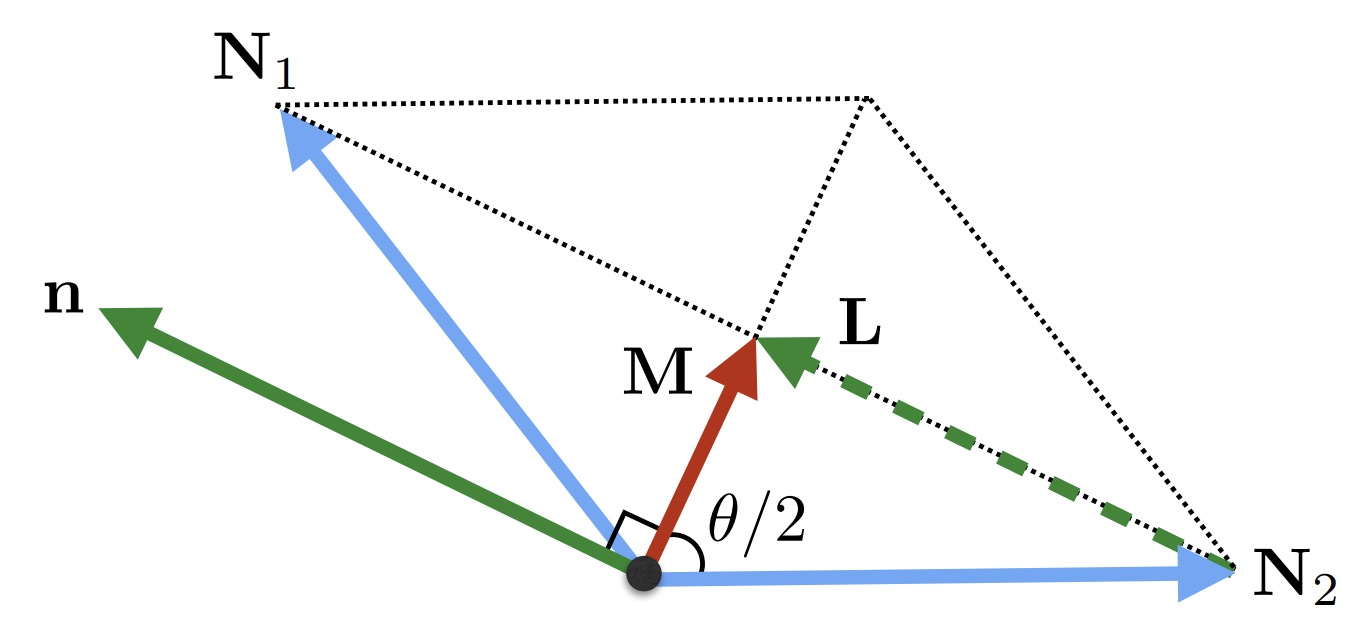
\includegraphics[scale=0.2]{Neel}
\caption{Decomposition of $\vec{N}_i$ into magnetic component $\vec{M}$ and Neel component $\vec{n}$ }
\end{figure}



\subsection{Antiferromagnetic system}
The discussion for spin waves in ferromagnetic systems is relatively straightforward, but it turns out that a lot more effort is needed to describe the spin waves in antiferromagnetic systems, as we have seen in the simple discussion for coupled spins above. \\

Here we consider a more concrete and useful example, where we have an infinite $d$-dimensional hypercubic lattice with antiferromagnetic nearest-neighbor exchange,
\begin{align*}
\hat{H} = \frac{J}{2}\sum_{\vec{j},\, \vec{a}} \hat{S}_{\vec{j}}\cdot \hat{S}_{\vec{j}+\vec{a}}\,,
\end{align*}
where we have $J>0$ indicating the antiferromagnetic configuration, $\vec{a}$ runs over all the nearest neighbors for site $\vec{j} = (j_1,\,j_2,\,\cdots,\,j_d) \in \Z^d$. If the ambient temperature is low, that is $k_\text{B}T \ll JS^2$, and the onsite spin $S$ is large, the spins must obey a good Neel order, at least locally, then it is Natural to write the onsite spin direction $\vec{N}$ as 
\begin{align*}
\vec{N}_{\vec{j}} = (-1)^{j_1 + j_2 + \cdots + j_d} \vec{n}_{\vec{j}}\sqrt{1 - a^{2d} m_j^2} + a^d\vec{m}_{\vec{j}}\,.
\end{align*}
Here $\vec{n}_{\vec{j}}$ is the dimensionless local Neel field which describes the overall orientation of neighboring spins (for each pair of neighboring spins, Fig.\,1 has $\vec{n}$ depicting the Neel component). $\vec{m}_{\vec{j}}$ is the local spin density, in units of $\hbar S$, which describes the relative canting of neighboring spins. They are defined in a way such that $$n_{\vec{j}}^2 = 1\,,\qquad \vec{n}_{\vec{j}}\cdot \vec{m}_{\vec{j}} = 0, \qquad\text{ and }(a^dm_{\vec{j}})^2 \ll 1\,,$$ which coincide with the intuition we developed in the previous section. This also guarantee that $$N_{\vec{j}}^2 = 1\,,\qquad \forall\vec{j}\,.$$ For a weakly-perturbed Neel texture, we can treat $\vec{n}_{\vec{j}}$ as varying smoothly in space-time and $\vec{m}_{\vec{j}}$ as small variable (as the total spin $\vec{M}$ for any neighboring pair is expected to be small in antiferromagnetic system). Then we can coarse-grained into $\vec{m}(\vec{r})$ and $\vec{n}(\vec{r})$ when taking the continuum limit. Alternatively, $\vec{n}(\vec{r})$ and $\vec{m}(\vec{r})$ can be defined via the following way: Antiferromagnet consists of two equivalent spin sublattices that are aligned antiparallel to each other in a classical ground state. We can develop a coarse-grained description starting with two smooth spin densities $\vec{m}_1(\vec{r})$ and $\vec{m}_2(\vec{r})$ of the two sublattices, such that $\vec{m}_1 \approx - \vec{m}_2$. Then the Neel field $\vec{n}$ and the net spin density $\vec{m}$ are defined as 
\begin{align*}
\vec{n}(\vec{r}) = \frac{\vec{m}_1(\vec{r}) - \vec{m}_2(\vec{r})}{|\vec{m}_1(\vec{r}) - \vec{m}_2(\vec{r})|}\,,\qquad
\vec{m}(\vec{r}) = \vec{m}_1(\vec{r}) + \vec{m}_2(\vec{r})\,.
\end{align*}

Now we can construct the discretized path-integral action for the antiferromagnetic spin lattice, following the spirit of equation (*) at the beginning of this section,
\begin{align*}
S = S_k + S_p = -\hbar S\int dt\,\sum_{\vec{j}}\int_0^1 du\, \vec{N}_{\vec{j}} \cdot \left( \pd_u \vec{N}_{\vec{j}}\times \pd_t \vec{N}_{\vec{j}}\right) - \frac{JS^2}{2}\sum_{\vec{j},\, \vec{a}}dt\, \vec{N}_{\vec{j}} \cdot \vec{N}_{\vec{j}+\vec{a}}\,.
\end{align*}
Here the cross-product term is the kinetic term, corresponding to the Wess-Zumino action $S_k$ on each site. The dot-product term is the potential term $S_p$, which is the negative of the Heisenberg interaction energy. Our goal is to simplify such an expression in the antiferromagnetic case. First we can utilize the new parametrization by the Neel field $\vec{n}$ and the net spin density $\vec{m}$. Let us start with the $S_p$ term, keeping the low-order terms,
\begin{align*}
\vec{N}_{\vec{j}} \cdot \vec{N}_{\vec{j}+\vec{a}} \approx - \vec{n}_{\vec{j}} \cdot \vec{n}_{\vec{j}+\vec{a}} + a^{2d}\vec{m}_{\vec{j}}\cdot \vec{m}_{\vec{j}+\vec{a}} + \frac{a^{2d}}{2}\left( \vec{m}_{\vec{j}}^2 + \vec{m}_{\vec{j}+\vec{a}}^2\right) \approx -\vec{n}_{\vec{j}} \cdot \vec{n}_{\vec{j}+\vec{a}} + 2a^{2d}\vec{m}_{\vec{j}}^2\,,
\end{align*}
where we have dropped terms linear in $\vec{m}$ as they shall get canceled once we sum over the lattice. Then for a smooth $\vec{n}(\vec{r})$, we consider writing (here for instance, $1$-dimensional lattice)
\begin{align*}
\vec{n}_{j+a} \approx \vec{n}_{j} + a\pd_i \vec{n}_{j} + \frac{a^2}{2}\pd_i^2 \vec{n}_j + \cdots\,.
\end{align*}
Also notice that $\vec{n}^2 = 1$ and thus $\vec{n}\cdot \pd_i \vec{n} = 0$, we can apply the trick 
\begin{align*}
\pd_i (\vec{n}\cdot \pd_i \vec{n}) = (\pd_i \vec{n})^2 + \vec{n}\cdot \pd_i^2 \vec{n} = 0\,,
\end{align*}
from which combining we obtain 
\begin{align*}
S_p \approx -\frac{1}{2}\int d^d r \int dt \,\left( K (\pd_i \vec{n})^2 + \frac{(\hbar S \vec{m})^2}{\chi}\right)\,,
\end{align*}
where again, only the lowest order terms are kept, and going from finite summing over $\vec{j}$ and $\vec{a}$ to the integral involves some coarse-grain. The coefficients that one should obtain from here are
\begin{align*}
K = JS^2 a^{2-d}\,,\qquad
\chi = \frac{\hbar^2}{4dJa^d}\,.
\end{align*}
A similar procedure can be done to the $S_k$ term, but before we do that, a notion of skyrmion should be introduced which will help us to investigate the topological contribution in the quantities. We shall do that in the next section. We will come back to this matter analyzing $S_k$ from the point of view of topological invariant in a later section. 


\section{Homotopy Groups and Skyrmions}
For this section,\footnote{Here is a very useful reference: Ji Zou's thesis on \textit{Aspects of magnetism: topology, transport, and quantum entanglement}.} we start by considering the definition of homotopy groups, which can be understood as a classification of ``holes" in a given manifold.\\

Given a topological manifold $X$, and a base point $x_0 \in X$, the first homotopy group $\pi_1(X,x_0)$ about $X$ at $x_0$ is also called the fundamental group. It can be understood as 
$$\pi_1(X,x_0)\coloneqq \{\text{loops\ }\gamma \text{ based at }x_0\} / \sim$$
where $\sim$ is the equivalent relation that can continuously transform the loops $\gamma$ from one to another. Here $\gamma:[0,1]\to X$ satisfies $\gamma[0] = \gamma[1] = x_0$ and needs to be continuous with respect to the topology defined on $X$. A homotopy is a continuous relation between the two loops $\gamma_1$ and $\gamma_2$, defining the equivalent relation $\sim$, which can be understood as a continuous map $h:[0,1]\times [0,1] \to X$ that satisfies
\begin{align*}
h(0,t)=h(1,t) = x_0 \ \forall t \in [0,1]\,,\qquad
h(r,0) = \gamma_1(r) \,,\ h(r,1) = \gamma_2(r)\ \forall r \in [0,1]\,.
\end{align*}
If such an $h$ exists, then $\gamma_1$ and $\gamma_2$ are said to be homotopic.\\

Since we are considering loops, elements in $\pi_1$ are loops, and it is not hard to see that $\pi_1$ has a group structure (composing two loops is just a larger loop which touches the base point three times when going from $t = 0$ to $t = 1$). For a concrete example, the fundamental group of $S^1$ at any base point is $\Z$, simply counting how many times $\gamma$ will warp around $S^1$ (with counterclockwise direction considered as positive count) when parametrized by $t \in [0,1]$. Thus, we write $\pi_1(S^1) = \Z$, regardless of the base point. In contrast, $\pi_1(S^2) = \{0\}$ is a trivial group, because all loops on $S^2$ can be shrunk to its base point via a continuous transformation. Lastly, $\pi_1(T^2)$ ($T^2$ is the donut-shape torus) is the free group generated by two elements, because there are two ways that one can wrap around a torus - either a long path around the whole torus or a short path around the ``tube."\\

\subsection{Spin winding}
Having this mathematical language established, we consider the first physical system here that can be described using the fundamental group. Consider a $1$-dimensional chain of spins $\{\vec{n}(r_i)\}$. Here we limit $\vec{n}(x_i) \in S^1$ for all $x_i$, and that $\vec{n}(\infty) = \vec{n}(-\infty)$ such that the two ends of the chain can be recognized as a single point. Essentially the parameter space for $\vec{n}$ can be viewed as $S^1$, and thus $\vec{n}$ can be viewed as a continuous map from $S^1$ to $S^1$. Thus, the different spin textures described by different $\vec{n}$ can be classified according to $\pi_1(S^1) = \Z$, and the integer number associated to the given $\vec{n}$ is called the topological charge for that spin texture. Mathematically, the topological charge number can be rigorously calculated via
\begin{align*}
N = \frac{1}{2\pi}\int \epsilon_{ab}n^a \pd_r n^b\, dr = \frac{1}{2\pi}\int \hat{z}\cdot \vec{n}\times \pd_r \vec{n}\, dr\,,
\end{align*}
where $a,b\in \{x,y\}$ are spatial indices for spatial components of $\vec{n}$ living in the $xy$-plane. One natural way to parametrize $\vec{n}$ is 
\begin{align*}
\vec{n}(r) = \bmat{\cos(\phi(r)) \\ \sin(\phi(r))}\,,
\end{align*}
in which case
\begin{align*}
N =\frac{1}{2\pi} \int \pd_r\phi \, dr\,.
\end{align*}
The conservation of a current 
\begin{align*}
j^\mu \coloneqq \frac{1}{2\pi} \epsilon^{\mu\nu}\pd_\nu \phi
\end{align*}
associated to such a topological charge then follows directly from such topological construction. Here $\epsilon^{\mu\nu}$ is the antisymmetric tensor with $\mu,\nu\in \{t,x\}$. \\

Notice that, we have been viewing $\pi(S^1)$ as an object that describes maps (the different textures $\vec{n}$) between $S^1$ and $S^1$ in this picture. This point of view is crucial in the rest of this section, where we will be classifying maps between $S^n$ and $S^m$ for given $n,m$ of interests. \\

\subsection{The structure of $\pi_2$ and $\pi_3$}
We have seen how $\pi_1$ is defined mathematically, and understood physically. For the main concerns in this note, we will focus only on homotopy groups $\pi_n$ for $n$ up to $3$. Let us build it up step-by-step. \footnote{For visualization and better understanding of homotopy groups, check out Dennis Sweeney's \textit{A Sphere is a Loop of Loops (Visualizing Homotopy Groups)} on \url{https://www.youtube.com/watch?v=CxGtAuJdjYI}.}\\

For a given topological manifold $X$, $\pi_2(X.x_0)$ at a base point $x_0 \in X$ concerns the classification of ``loop of loops." Here we will make it more precise. Let $\Omega(X,x_0)$ denote the set of loops on $X$ based at $x_0$, then 
\begin{align*}
\pi_2(X,x_0) \coloneqq \Omega(\Omega(X,x_0), \, \gamma_0) / \sim\,,
\end{align*}
where $\gamma_0$ denotes the constant map in $\Omega(X,x_0)$, and $\sim$ is the equivalent relation defined by a continuous map between $\kappa_1$ and $\kappa_2$ in $\Omega^2(X,x_0) \coloneqq \Omega(\Omega(X,x_0), \, \gamma_0)$. This is abstract but it is indeed a classification of ``loop of loops." One key observation here is that $\gamma_0$ is a constant map, that is $\gamma_0(t) = x_0$ for all $t \in [0,1]$. Thus, each element in $\Omega^2(X,x_0)$ can be considered as: A size-changing loop that is moving in space, with one point fixed at $x_0$, such that at $t = 0$, the entire loop is shrunk at $x_0$, then at a later time $0<t <1$, the loop is enlarged, moving through the space on $X$, and at the end at $t = 1$, the loop shrinks back to the single point at $x_0$. This size-changing moving loop, parametrized by time, sweeps out a sphere-like object. In fact, $\kappa(s)(t) \in X$ for $\kappa \in \Omega^2(X,x_0)$ and $s,t \in [0,1]$, where $s,t$ can be understood as the latitude and longitude coordinates on the sphere that $\kappa$ sweeps out, because $\kappa(s)(t) = x_0$ if either or both $s,t\in\{0,1\}$. \\

Therefore, if $X = S^2$ is the manifold of interest, $\kappa$ can be understood as mapping between $S^2$ (a parameter space) and $S^2$ (a target space). In this sense, $\kappa \in \Omega^2(S^2,x_0)$ for any $x_0 \in S^2$ can be viewed as an object that wraps $S^2$ an integer number of times, such that we get $\pi_2(S^2) = \Z$. From her it is also not difficult to see that $\pi_2(S^1) $ is a trivial group, and $\pi_2(S^3)$ is also a trivial group. \\

Summarizing here, $\pi_1$ can detect loop-like ($S^1$-like) holes in a topological manifold, and $\pi_2$ can detect sphere-like ($S^2$-like) holes. This idea, and the idea of ``loop of loops" can be generalized further. The definition of $\pi_3$ then follows, 
\begin{align*}
\pi_3(X,x_0) \coloneqq \Omega(\Omega(\Omega(X,x_0), \kappa_0)/\sim\, \coloneqq \Omega^3(X,x_0)/\sim\,, 
\end{align*}
where again $\kappa_0$ denotes a constant map in $\Omega^2(X,x_0)$, and $\sim$ is a equivalent relation defined by continuous deformation between maps in $\Omega^3(X,x_0)$. $\pi_3$ detects $S^3$-ilke holes, and $\pi_3(S^3) = \Z$. \\

As we have seen that $\pi_2$ describes ``loop-of-loops" objects, we can think of $\pi_3$ describing ``loop-of-spheres" objects, or size-changing spheres. In this sense, we can consider how to use a size-changing sphere-like object to wrap around $S^2$. Pictorially this can be viewed as stuffing a ping-pong ball in a balloon (from outside of the balloon) - a small portion of the balloon will wrap the ping-pong ball, and we can also twist that small portion of the balloon multiple times to wrap the ping-pong ball more tightly. From this point of view, the number of time that we twist is an integer number, and therefore we purpose $\pi_3(S^2) = \Z$. In contrast with $\pi_2(S^1)= \{0\}$. Lastly, it is not hard to verify that $\pi_3(S^1) = \{0\}$. This concludes our intro-level discussion about the structure of $\pi_2$ and $\pi_3$.

\subsection{Skyrmion and hedgehog}
Again, having the mathematical language established, we can talk about the physical picture. First we introduce the $2$-dimensional skyrmion, which are classified by $\pi_2(S^2)$. Therefore, we are interested in a unit vector field $\vec{n}:\R^2 \to S^2$, and we require that 
\begin{align*}
\lim_{|\vec{r}|\to\infty}\vec{n}(\vec{r}) = \vec{n}_0
\end{align*}
to be a constant such that the spin texture at infinity (in all directions) can be recognized as a single vector on $S^2$, which compactifies $\R^2$ into $S^2$. Thus $\vec{n}$ is essentially a map between $S^2$ and $S^2$, following the discussion of $\pi_2$ we see that $\vec{n}$ in this case is naturally classified by $\pi_2$. The topological charge is then defined as
\begin{align*}
N = \frac{1}{4\pi}\int \epsilon_{abc} n^a \pd_x n^b \pd_y n^c \, dx\, dy = \frac{1}{4\pi}\int \vec{n}\cdot \pd_x \vec{n}\times \pd_y \vec{n}\, dx\, dy\,,
\end{align*}
with $a,b,c\in\{x,y,z\}$, and the current associated to such a $2$-dimensional skyrmion is defined as
\begin{align*}
j^\mu = \frac{1}{4\pi}\epsilon^{\mu\nu\rho} \vec{n}\cdot (\pd_{\nu} \vec{n}\times \pd_{\rho} \vec{n})\,,
\end{align*}
with $\mu,\nu,\rho \in\{t,x,y\}$. The conservation of the current follows directly from the antisymmetric property of $\epsilon^{\mu\nu\rho}$, 
\begin{align*}
\pd_\mu j^\mu = 0\,.
\end{align*}

Hedgehog is defined similarly to the $2$-dimensional skyrmion, with the only difference being the parameter space for $\vec{n}$. In the case of hedgehog, we consider $\vec{n}: \R^3 \to S^2$. Then we focus on a base point $\vec{r}_0 \in \R^3$, and we construct a sphere $S^2_0$ around the base point $\vec{r}_0$. The spin texture $\vec{n}|_{S^2_0}$ on the sphere is a map from $S^2$ to $S^2$, and is thus classified by $\pi_2$. The $2$-dimensional skyrmion measures the topology on the whole space, whereas the $3$-dimensional hedgehog measures the topology on a ``point defect" in space. \\

A $3$-dimensional skyrmion concerns $\pi_3(S^3) = \Z$, so we are interested in $\vec{n}: \R^3 \to S^3$, with the compactification of $\R^3$ into $S^3$ by the addition of the point at infinity. In the language of low energy description of QCD, the target space is SU$(2)$, viewed as $S^3$, and the parameter space is $\R^3$ with one-point compactification. In this case, we define topological charge
\begin{align*}
N = \frac{1}{12\pi^2} \int d^3r \, \epsilon_{ijk}\,\epsilon_{abcd} \, n_a\,\pd_i n_b\, \pd_jn_c \, \pd_k n_d\,,
\end{align*}
with the conserved current
\begin{align*}
j^\mu \propto \epsilon^{\mu\nu\rho\kappa} \epsilon_{abcd}\, n_{a} \, \pd_\nu n_b \, \pd_\rho n_c \, \pd_\kappa n_d\,,
\end{align*}
with $\mu,\nu,\rho, \kappa \in \{t,x,y,z\}$; $i,j,k\in\{x,y,z\}$; and $a,b,c,d \in \{x_1,x_2,x_3,x_4\}$. 

\section{Magnetic Helicity and Hopfion}
There is one homotopy group classification in the previous section that we have introduced in the language of mathematics, but have not yet revealed its physical representation - the group of $\pi_3(S^2) = \Z$ - a homotopy group that is particularly difficult to visualize comparing to the other ones discussed. We will explore more about the structure of this group in this section. \footnote{Here are some very useful references: Mitchell Berger's paper on \textit{Introduction to magnetic helicity}; Ross Knapman's paper on \textit{Spacetime magnetic hopfions from internal excitations and braiding of skyrmions}.}\\

Let us start by considering magnetic flux tubes, from which we can construct magnetic helicity, a topological structure of magnetic field lines. Consider two closed curves $\vec{x}(\sigma)$ and $\vec{y}(\tau)$ (also labeled by $1$ and $2$, respectively), and let $\vec{r} = \vec{y}-\vec{x}$, the Gauss linking number associated to these two curves is 
\begin{align*}
L_{12} = -\frac{1}{4\pi}\oint_1 \oint_2 \frac{d\vec{x}}{d\sigma}\cdot \left( \frac{\vec{r}}{r^3} \times \frac{d\vec{y}}{d\tau}\right) \, d\tau	\, d\sigma\,. \tag{*}
\end{align*}
Here $L_{12}$ is an integer number counting the number of times the two curves are linked. We will want to use such a definition of linking number to describe the ``linking" of magnetic field lines (or flux tubes). \\

Suppose we can approximate a magnetic field in a closed simply-connected volume $V$ by a collection of flux tubes, such that 
\begin{align*}
\vec{B}\cdot \hat{n}|_S = 0 \tag{$\dagger$}
\end{align*}
along the boundary $\pd V = S$. Here the requirement of simply connectedness of the domain $V$ is enforced, such that all the allowed gauge transformation of the vector potential $\vec{A}$ for describing the given magnetic field $\vec{B} = \nabla \times \vec{A}$ satisfies $\vec{A} \to \vec{A} + \nabla f$ for some scalar function $f$.\\

Let there be $N$ tubes and the fluxes carried by each is denoted as $\Phi_i$, then we can compute
\begin{align*}
K = \sum_i \sum_j L_{ij} \Phi_i \Phi_j\,,
\end{align*}
with $L_{ij}$ calculated via (*). Taking $N \to \infty$ and $\Phi_i \to 0$, and realizing we have locally $\Phi_i \, d\vec{l}_i = \vec{B}(\vec{x})\, d^3x$, we obtain 
\begin{align*}
K = -\frac{1}{4\pi}\int \int \vec{B}(\vec{x}) \cdot \left( \frac{\vec{r}}{r^3} \times \vec{B}(\vec{y})\right) \, d^3x \, d^3y\,,\tag{**}
\end{align*}
where $\vec{r} = \vec{y} - \vec{x}$. Here $K$ is understood as the total linkage of the magnetic field lines, or the total linkage of the flux tubes weighted by the magnetic flux they are carrying. We can write (**) in a particularly nicer form using the Coulomb gauge vector potential 
\begin{align*}
\vec{A}(\vec{x}) = -\frac{1}{4\pi}\int \frac{\vec{r}}{r^3} \times \vec{B}(\vec{y}) \, d^3y\,,
\end{align*}
such that 
\begin{align*}
K = \int \vec{A}\cdot \vec{B}\, d^3x\,. \tag{***}
\end{align*}
Notice that however, $K$ is not integer-valued - it has a unit of [flux$^2$], and is thus weighted by the flux (strength of magnetic field) in the region.\\

Another key observation here is that, even we employed the Coulomb gauge in the derivation from (**) to (***), we should note that (***) is independent on the gauge choice as long as the boundary condition satisfies ($\dagger$).  To see this, given that ($\dagger$) holds, consider $\vec{A} \to \vec{A} + \nabla f$, then
\begin{align*}
\Delta K = \int_V(\nabla f) \cdot \vec{B} \, d^3x = \oint_{S} f\,\vec{B}\cdot \vec{n} \, dS = 0\,.
\end{align*}
Furthermore, here we have taken the assumption that $V$ is simply connected, otherwise there can exist a vector field $\vec{G}$ such that $\nabla \times \vec{G} = 0$ (so that it can be viewed as a gauge transformation $\vec{A} \to \vec{A} + \vec{G}$) but $G \neq \nabla f$ for any scalar-valued $f$, in a multiply connected domain (for instance, a torus). \\

Essentially, (***) serves as our definition of $K$, and it makes it easier to understand what $K$ is when we employ the Coulomb gauge to establish its connection to (**), which recovers the familiar integral used for computing the Gauss linking number of the magnetic flux lines. \\

Before we discuss how to deal with different boundary conditions and relaxing the requirement of having a simply connected domain, let us introduce the idea of hopfion, and see how magnetic helicity introduced above can help us to understand hopfion.\\

A hopfion is a nonlinear texture $\vec{n}:\R^3 \to S^2$ classified by the homotopy group $\pi_3(S^2) = \Z$. The parameter space $\R^3$ is viewed as $S^3$ via one-point compactification -  the infinity points are identified as one point by having 
\begin{align*}
\lim_{|\vec{r}|\to \infty}\vec{n}(\vec{r}) = \vec{n}_0
\end{align*}
being a constant. The hopf index associated to such a texture is defined as
\begin{align*}
Q = -\int d^3r \,\mathcal{\vec{A}}\cdot \mathcal{\vec{B}}\,, \tag{$\square$}
\end{align*}
with
\begin{align*}
\mathcal{B}_i \coloneqq \frac{1}{8\pi}\epsilon_{ijk}\vec{n}\cdot \pd_j\vec{n}\times \pd_k \vec{n}
\end{align*}
and $\mathcal{\vec{A}}$ being the associated vector potential such that $\nabla\times \vec{\mathcal{A}} = \mathcal{\vec{B}}$. We require the assumption that $\vec{n}$ is smooth enough such that $\nabla \cdot \vec{\mathcal{B}} = 0$. The negative sign in ($\square$) is required for matching the conventional Hopf map orientation. Here we see that the definition of the topological invariant, the hopf charge, in ($\square$) matches with the definition of magnetic helicity in (***), with the only difference arising from the physical meaning of the field $\mathcal{\vec{B}}$ (or $\vec{B}$). It follows from the previous discussion that $Q$ should be gauge invariant, as the space $S^3$ (or $\R^3$ with one-point compactification) which defines $\mathcal{\vec{B}}$ is simply connected, and $\mathcal{\vec{B}}(\vec{r})\to 0$ as $|\vec{r}| \to 0$. \\

Even $K$ is in general non-integer-valued, here $Q$ is in fact integer-valued. This is because $\vec{\mathcal{B}}$ has a built-in normalization via its definition, while $\vec{B}$ as a magnetic field in calculating magnetic helicity is in general not normalized. The details of such a normalization fixes the integer-valued nature of $Q$ involves viewing $\mathcal{\vec{B}}$ as the pullback of the area form on $S^2$, but we can also try to understand this idea more intuitively, by recalling the linking number description in magnetic helicity. Here the preimage of a given $\vec{n}_a \in S^2$ by $\vec{n}$ is a loop (or some loops, here WLOG we assume the preimage of $\vec{n}_a$ is only one loop) in $S^3$. For a given pair of $\vec{n}_a, \vec{n}_b \in S^2$, we obtain a pair of loops via preimaging them by the map $\vec{n}$ (again, we assume $\vec{n}^{-1}(\vec{n}_b)$ is also a single loop), and the Gauss linking number of the pair of loops can be computed. Due to the continuity of $\vec{n}$, continuously moving $\vec{n}_a$ and $\vec{n}_b$ on $S^2$ will deform the their preimaged loops in $S^3$ continuously, thus the linking number calculated via preimaging $\vec{n}_a$ and $\vec{n}_b$ in fact does not depend on the based points $\vec{n}_a$ and $\vec{n}_b$ chosen on $S^2$, and it depends only on the structure of $\vec{n}$. Here we can conclude that, for any pair of points on $S^2$, the linking number $L$ of the loops generated by preimaging the points via $\vec{n}$ is the same. In fact, we have $Q = L$, which can be seen by utilizing the Coulomb gauge which defines $\vec{\mathcal{A}}$ to arrive
\begin{align*}
Q = \frac{1}{4\pi}\int \int \vec{\mathcal{B}}(\vec{x}) \cdot \left( \frac{\vec{r}}{r^3} \times\vec{\mathcal{B}}(\vec{y})\right) \, d^3x \, d^3y\,.\tag{$\boxminus$}
\end{align*}
Here ($\boxminus$) resembles the helicity expression that sums pairwise linkings of flux elements, but in fact $\mathcal{\vec{B}}$ has done the job of normalization such that $Q $ is the linking number of loops generated by preimaging any pair of points in $S^2$.\footnote{For more details, check out Chern–Simons functional and hopf fibration.}

\section{Transport of Magnetic Helicity}
In the previous section, we have argued that the magnetic helicity is gauge invariant if the space of domain is simply connected and the boundary condition $\vec{B} \cdot \hat{n}|_S = 0$ is satisfied. However, field lines can terminate at the boundary in physical setups, and the domain space is not necessarily simply connected either. These considerations motivate a general definition of helicity integral, where we will the field into a vacuum part and a closed part, following the analysis by Berger in section 3 of his paper \textit{Introduction to magnetic helicity}.\\



\chapter{-}
\section{Input-output formalism}

\section{Landau-Lifshitz-Gilbert Equation}



\end{document}
 





